パラ言語情報に関する研究は、人と人とのコミュニケーションに関与していながら従来十分には注意が払われてこなかった要素を解明することで、音声コミュニケーション過程に対する我々の理解を深化させることができる\cite{maekawa_kitagawa}


多様な関係性の音声に含まれる

%--------------------
\begin{figure}[hbtp]
 \centering
   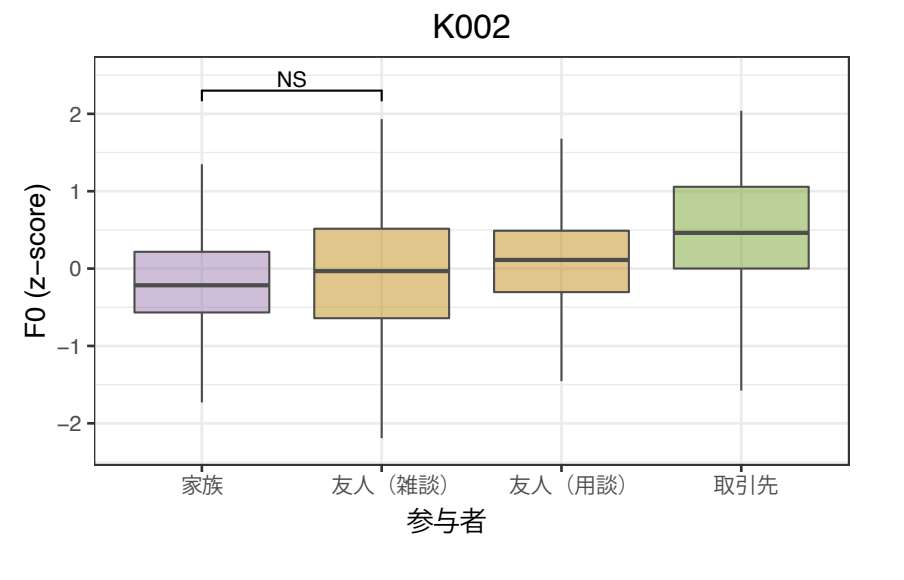
\includegraphics[width=12.0cm]{figures/ishimoto2.png}
 \caption[発話者K002(女性)のFoと会話場面の参与者との関係]{発話者K002(女性)のFoと会話場面の参与者との関係。 \cite{ishimoto}より抜粋。 }
 \label{ishimoto2:fig}
\end{figure}

%--------------------

表
\begin{table}[htb]
    \begin{center}
    \caption{各組織において定義されている声質}
    \label{tb:around_voice_quolity}
        \begin{tabular}{|ll|} \hline
            組織                                                 & 声質                           \\ \hline \hline
            日本音声言語医学会: GRBAS尺度 ~\cite{vq_9}           & Grade: 総合的な嗄声度          \\
            動画で見る音声障害(DVD) ~\cite{vq_10}で訓練可能      & Rough: 粗そう性                  \\
                                                                 & Breathy: 気息性                \\
                                                                 & Asthenic: 無力性               \\
                                                                 & Strained: 努力性               \\ \hline
            国際音声学会(IPA): IPA の定める声質 ~\cite{vq_2}     & Falsetto: 裏声                 \\
                                                                 & Whispery: ささやき声           \\
                                                                 & Breathy: 息漏れ声              \\
                                                                 & Creaky: きしみ声,パルス的な声 \\
                                                                 & Harsh: 耳障りな音              \\ \hline
            John Laver: 声帯振動のモードによる分類 ~\cite{vq_11} & Modal: 地声                    \\
                                                                 & Falsetto: 裏声                 \\
                                                                 & Whisper: ささやき声            \\
                                                                 & Creak: きしみ声、パルス的な声  \\
                                                                 & Harshness: 耳障りな声、りきみ音\\
                                                                 & Breathiness: 息漏れ声          \\ \hline
        \end{tabular}
    \end{center}
\end{table}